\uuid{jJh4}
\exo7id{5816}
\auteur{rouget}
\organisation{exo7}
\datecreate{2010-10-16}
\isIndication{false}
\isCorrection{true}
\chapitre{Conique}
\sousChapitre{Conique}

\contenu{
\texte{
Etudier les courbes dont une équation polaire (en repère orthonormé direct) est
}
\begin{enumerate}
    \item \question{$r =\frac{2}{1-2\cos\theta}$,}
\reponse{$e = 2$. Il s'agit une hyperbole dont l'un des foyers est l'origine.


$$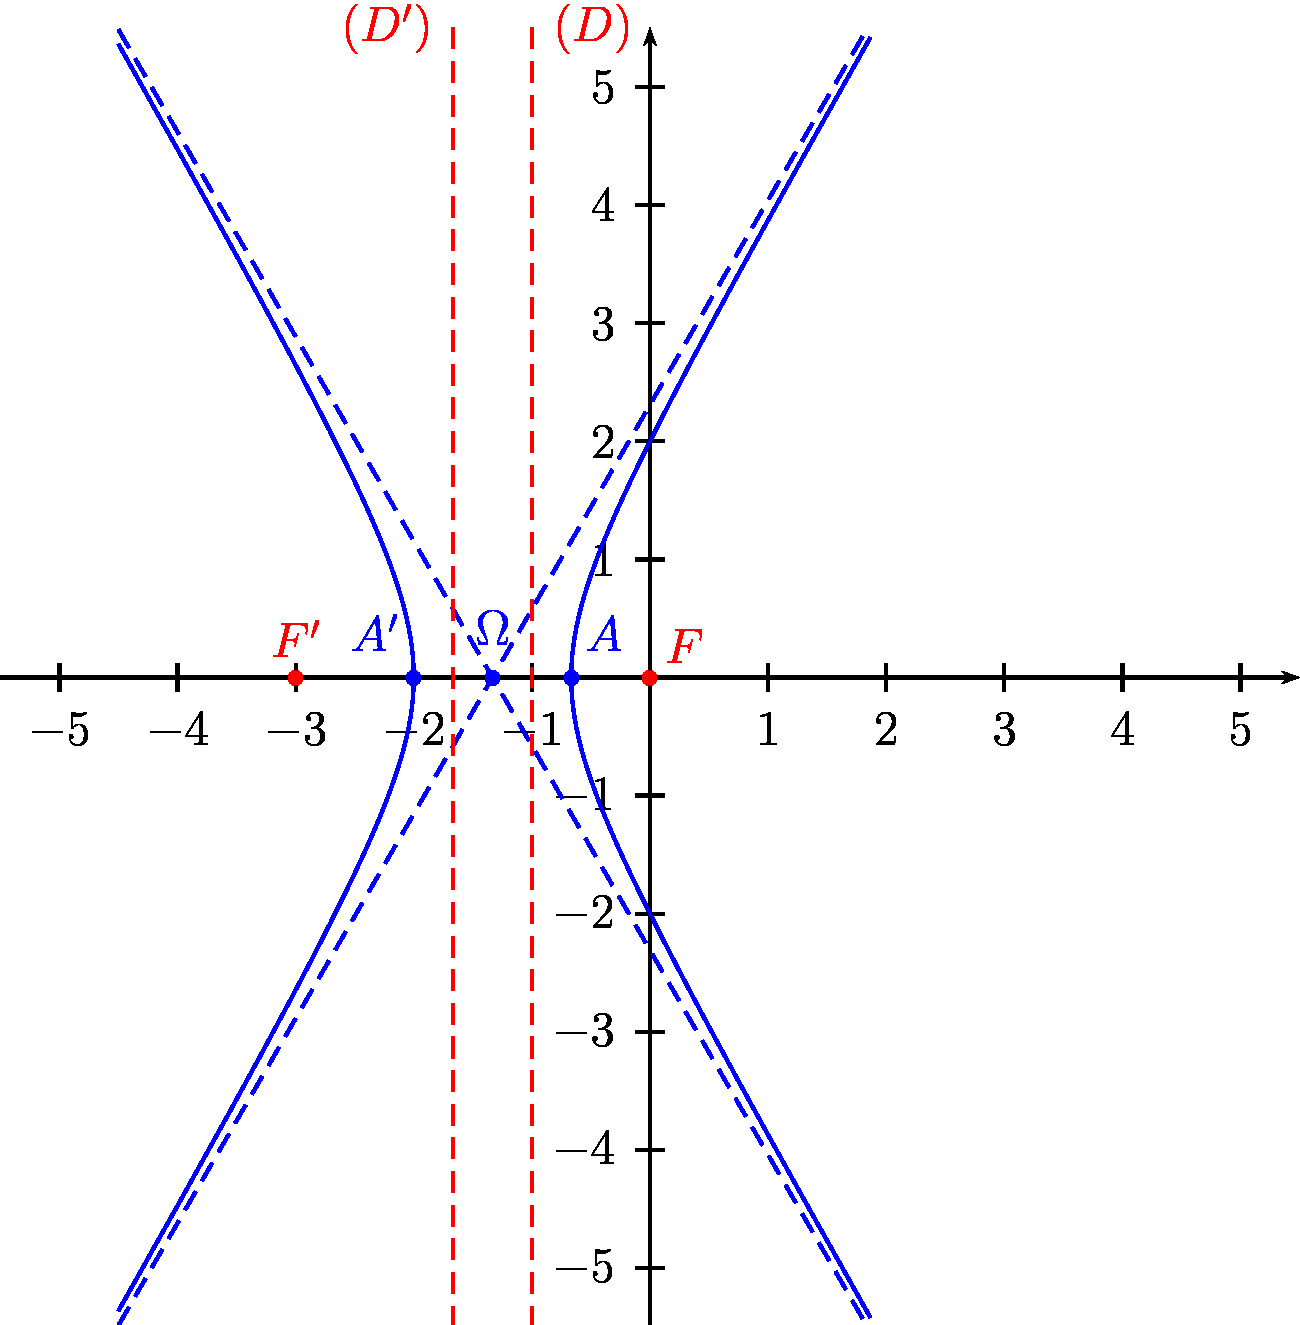
\includegraphics{../images/img005816-1}$$



L'axe focal est $(Ox)$ et donc les sommets de l'hyperbole sont les points d'intersection de la courbe avec l'axe $(Ox)$. Ce sont les points $A$ et $A'$ de coordonnées cartésiennes $\left(-\frac{2}{3},0\right)$ et $(-2,0)$ obtenus pour $\theta=\pi$ et $\theta=0$ respectivement.

Le centre est le milieu du segment $[AA']$ à savoir le point $\Omega\left(-\frac{4}{3},0\right)$.

les directions asymptotiques sont fournies par : $2\cos\theta- 1 = 0\Leftrightarrow\theta\in\pm\frac{\pi}{3}+2\pi\Zz$. Les asymptotes sont les droites d'angle polaire $\pm\frac{\pi}{3}$ passant par $\Omega$. Ce sont les droites d'équations respectives $y =\sqrt{3}\left(x+\frac{4}{3}\right)$ et $y = -\sqrt{3}\left(x+\frac{4}{3}\right)$.

L'un des foyers $F$ est l'origine. L'autre est le symétrique de $F$ par rapport à $\Omega$ à savoir  le point $F'$ de coordonnées $(-3,0)$.

Les directrices sont fournies par les points $K =\Omega+\frac{1}{e}\overrightarrow{OA}=(-1,0)$  et 
$K'=\Omega-\frac{1}{e}\overrightarrow{OA}=\left(-\frac{5}{3},0\right)$. Les directrices sont les droites $(D)$ et $(D')$ d'équations respectives $x = -1$ et $x=-\frac{5}{3}$.}
    \item \question{$r =\frac{6}{2+\cos\theta}$,}
\reponse{L'équation s'écrit $r=\frac{3}{\frac{1}{2}+\cos\theta}$. Donc $e =\frac{1}{2}$ et la courbe est une ellipse.

$$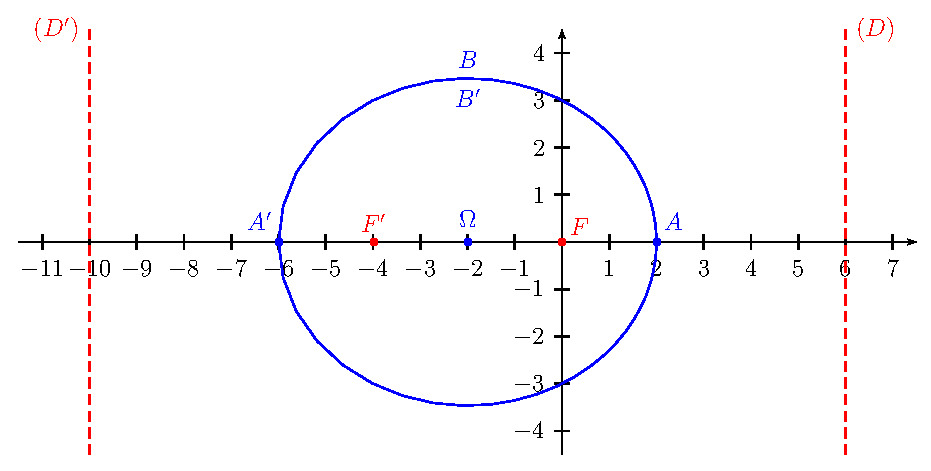
\includegraphics{../images/img005816-2}$$


Les sommets du grand axe sont les points $A(2,0)$ et $A'(-6,0)$ obtenus pour $\theta=0$ et $\theta=\pi$. Le centre est le milieu $\Omega$ de $[AA']$ de coordonnées $(-2,0)$.

Le premier foyer $F$  est l'origine et le deuxième est le symétrique du point $F$ par rapport à $\Omega$ à savoir le point $F'(-4,0)$.

Les points $K$ et $K'$ sont définis par : $K = \Omega+\frac{1}{e}\overrightarrow{OA}=(6,0)$   et 
$K'= \Omega-\frac{1}{e}\overrightarrow{OA}=(-10,0)$. Les directrices sont les droites $(D)$ et $(D')$ d'équations respectives $x = 6$ et $x = -10$.

Les sommets du petit axe sont déterminés par $b=\sqrt{a^2-c^2}=\sqrt{4^2 - 2^2}=\sqrt{12}$ puis 
$B=\Omega+b\overrightarrow{j}=\left(-2,2\sqrt{3}\right)$ et $B=\Omega-b\overrightarrow{j}=\left(-2,-2\sqrt{3}\right)$}
    \item \question{$r =\frac{2}{1-\sin\theta}$.}
\reponse{L'équation $r=\frac{2}{1+\cos\left(\theta+\frac{\pi}{2}\right)}$. On reconnait une parabole dans une présentation non traditionnelle.

Le foyer est toujours l'origine et comme la direction asymptotique est obtenue pour $\theta=\frac{\pi}{2}$ (et a donc pour angle polaire $\frac{\pi}{2}$), l'axe focal est donc la droite passant par l'origine $F$ et d'angle polaire $\frac{\pi}{2}$, c'est-à-dire l'axe des ordonnées. Le sommet est l'intersection de la courbe avec l'axe $(Oy)$ obtenue pour $\theta=-\frac{\pi}{2}$. Pour $\theta=-\frac{\pi}{2}$, on obtient $r=1$ et donc $S(-1,0)$. Puis $K =s_S(F) =(-2,0)$ et la directrice $(D)$ est la droite d'équation $y = -2$. Enfin, $p=FK= 2$.

$$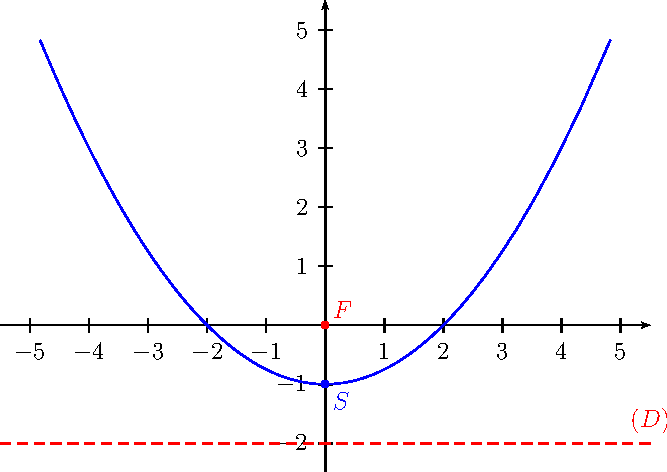
\includegraphics{../images/img005816-3}$$


\textbf{Remarque.} Si on n'est pas à l'aise en polaires, on peut toujours repasser en cartésien mais c'est une très grosse perte de temps :

En 1), $r(1-2\cos\theta) = 2$ s'écrit $r -2x = 2$ puis $x^2+y^2 = (2x+2)^2$.

En 2), $r(2+\cos\theta) = 6$ s'écrit $2r + x = 6$ et donc $4(x^2+y^2) =(-x+6)^2$.

En 3), $r(1-\sin\theta) = 2$ s'écrit $r - y = 2$ puis $x^2+y^2 = (y+2)^2$ et donc $y=\frac{x^2}{4}-1$.}
\end{enumerate}
}
